\documentclass[12pt,letterpaper]{article}

%\usepackage{fontspec}
%\usepackage[utf8]{inputenc}
\usepackage{textcomp,marvosym}
\usepackage{amsmath,amssymb}
\usepackage[left]{lineno}
\usepackage{changepage}
\usepackage{rotating}
\usepackage{natbib}
\usepackage{setspace} 
\usepackage{lastpage}
\usepackage{fancyhdr}
\usepackage{graphicx}
\usepackage{wrapfig}
\usepackage{hyperref}
%\doublespacing

\raggedright
\textwidth = 6.5 in
\textheight = 8.25 in
\oddsidemargin = 0.0 in
\evensidemargin = 0.0 in
\topmargin = 0.0 in
\headheight = 0.0 in
\headsep = 0.5 in
\parskip = 0.05 in
\parindent = 0.1in

% Bold the 'Figure #' in the caption and separate it from the title/caption with a period
% Captions will be left justified
%\usepackage[aboveskip=1pt,labelfont=bf,labelsep=period,justification=raggedright,singlelinecheck=off]{caption}

% Remove brackets from numbering in List of References
%\makeatletter
%\renewcommand{\@biblabel}[1]{\quad#1.}
%\makeatother

\pagestyle{myheadings}
\pagestyle{fancy}
\fancyhf{}
\lhead{Fairchild} 
\chead{\textit{Flexural and thermal subsidence of the Midcontinent Rift}}
\rhead{\thepage/\pageref{LastPage}}

\renewenvironment{abstract}
 {\small
  \begin{center}
  \bfseries \abstractname\vspace{-.5em}\vspace{0pt}
  \end{center}
  \list{}{
    \setlength{\leftmargin}{.5cm}%
    \setlength{\rightmargin}{\leftmargin}%
  }%
  \item\relax}
 {\endlist}


%\documentclass[12pt,a4paper]{article}
\usepackage[a4paper, margin=1.0in]{geometry}
\usepackage{siunitx}
\usepackage{textcomp}

\begin{document}\thispagestyle{empty}
\begin{flushleft}
{\Large \textbf{Flexural and thermal subsidence of the 1.1 Ga Midcontinent Rift}}\\
\vspace{0.3em}
Luke Fairchild, EPS 108 Term Paper --- 12/15/2015
%Luke M. Fairchild\textsuperscript{1,2},
%Nicholas L. Swanson-Hysell\textsuperscript{1},
%Sonia M. Tikoo\textsuperscript{1,3}
%\title{Modeling the flexural and thermal subsidence of the 1.1 Ga Midcontinent Rift}
%\author{Luke Fairchild}
%\begin{document}
%\maketitle{}
\end{flushleft}

\begin{abstract}
\hline
The Midcontinent Rift (MCR) is a failed rift system that formed within the interior craton of Laurentia (Mesoproterozoic North America) and was active from $\sim$1110 to 1085 Ma. 
%The MCR is notable in both its total volcanic output, which qualifies it as a large igenous province ($\geq$\SI{e5}{km^3} by the criterion of Ernst et al., 2013\nocite{Ernst2013b}), and its geometry, which qualifies it as a rift system. These two characteristics, while present together in the MCR, are not typically associated with each other as they are thought to derive from separate mechanisms. The MCR is therefore of great interest from a standpoint of geodynamics. No consensus has yet been reached on the geodynamic evolution and tectonic history of this ancient system.\par
%While the volume of volcanic rock in the MCR ($\sim$1-\SI{2e6}{km^3}; \cite{Hutchinson1990a}) necessitates a mantle plume origin, it is unclear whether the plume had any role in the initiation of the rift itself. Recent studies suggest that the MCR formed in response to far-field tectonic stresses as Amazonia rifted from Laurentia, and ended once oceanic spreading between the two continents was successfully established \cite{Stein2014a}. This hypothesis further interprets the MCR as a rift system that coincidentally encountered a mantle plume capable of generating LIP flood basalts, consistent with the idea that the small temperature perturbations ($\sim$100-150\textdegree\ C above normal mantle temperatures) of hotspots can dramatically amplify the decompression magmatism of rift zones \cite{White1989a}. In order to resolve the broad-scale geodynamics of this LIP/rift duality, it becomes important to better understand the wholesale development of the MCR.\par{}
A widely accepted timeline of MCR development has been inferred through seismic, geochemical, geochronologic and structural measurements \citep{Cannon1989a,Cannon1992b,White1997a,Stein2015a}. The syn- and post-rift flexural and thermal subsidence of the MCR is the least constrained stage of rift development, as sediments are the primary lithological product of this period and generally have not yielded reliable dates. Understanding the timeline and nature of MCR subsidence is critical for inferring past structure and rift duration from present observations. This study compiles and reviews the estimates of past investigations of MCR subsidence in the context of the MCR's broader developmental timeline. In doing so, I aim to give a comprehensive overview of the MCR system similar to that presented by Stein et al. (2015) but with a specific focus on the MCR's subsidence history.
\vspace{0.5em}\hline
\end{abstract}

\section{INTRODUCTION}
The Mesoproterozoic Midcontinent Rift (MCR) is the most prominent feature on gravity and magnetic maps of North America. The MCR primarily consists of thick flood basalt successions confined to a narrow zone extending northward from the Midwestern United States into Lake Superior and looping back southward through Michigan, U.S (Fig. \ref{fig:MCR_fig}). 
\begin{wrapfigure}{r}{0.5\textwidth}
\noindent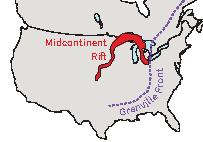
\includegraphics[width=0.5\textwidth]{figures/MCR_fig.pdf}
\caption{\footnotesize{Location and outline of the Midcontinent Rift and the Grenville Front.}}
\label{fig:MCR_fig}
\end{wrapfigure}
The origin of the MCR is an outstanding question in current investigations. While the volume of volcanic rock in the MCR ($\sim$1-\SI{2e6}{km^3}; Hutchinson et al., 1990\nocite{Hutchinson1990a}) necessitates a mantle plume origin ($\geq$\SI{e5}{km^3} by the criterion of Ernst et al., 2013\nocite{Ernst2013b}), it is unclear whether the plume had any role in the initiation of the rift itself. Recent studies suggest that the MCR formed in response to far-field tectonic stresses as Amazonia rifted from Laurentia, and ended once oceanic spreading between the two continents was successfully established \citep{Stein2014a}. This hypothesis of an already active rift encountering a mantle plume by chance is consistent with the idea that the small temperature perturbations ($\sim$100-150\textdegree\ C above normal mantle temperatures) of hotspots can dramatically amplify the decompression magmatism of rift zones \citep{White1989a}. Constraining the geodynamic evolution of the MCR is critical for 1) evaluating the feasibility of such hypotheses in the context of rift basin development, 2) understanding potential unique structural consequences of interaction between continental rifting and a mantle plume, and 3) constraining the dynamics of post-rift sedimentation.\par

\cite{Cannon1992a} used seismic data across Lake Superior to map the structure of the MCR and infer discrete stages of faulting and volcanism. The conclusions of this study are widely accepted as the general timeline of the MCR's geodynamic evolution, which is outlined here. At $\sim$1110 Ma, rifting and incipient volcanism occurred, followed by an outburst of ``main" stage flood basalts confined to the central graben until $\sim$1095 Ma. Continued ``late" stage volcanism resulted in further flexural subsidence and subsequent sedimentation. While it has been proposed that crustal thickening also occurred during this last stage of rifting \citep{Stein2015a}, it is plausible that significant thermal subsidence (cooling and thickening of the lithosphere) would have been prevented or delayed by the elevated temperatures and forces of an upwelling mantle plume \citep{White1997a}. Rifting ended at $\sim$1085 due to either far-field tectonic stresses (both compressional and extensional events have been proposed; \cite{Stein2014a,Cannon1994a}) or the dissipation or relocation of the mantle plume source in the presence of fast plate tectonic rates \citep{Swanson-Hysell2014a}. By this time, thermal subsidence would have certainly been underway. The cumulative post-rift subsidence in the MCR would have dramatically altered the surface long after the rifting had actually ceased, a factor that must be considered in interpretations of the rift's evolution and tectonic setting.\par

Constraining this post-rift stage of MCR development is paramount to a comprehensive understanding of this unique geologic feature. Additionally, in the absence of coherent age constraints on MCR sediments, quantifying expected subsidence and associated sedimentation in the MCR could allow a better understanding of syn- and post-rift sedimentary sequences and the timeframe and geologic context of their deposition. For example, recent detritial zircon dates from the post-rift Jacobsville sandstone suggest that this 3-4 km thick sedimentary infill was still being deposited at $\sim$900 Ma \citep{Craddock2013a}, much later than the Grenville orogeny that presumably interrupted the development of the post-rift sedimentary basin. While this particular data is under immense scrutiny, it demonstrates how such findings cannot yet be robustly tested (and possibly dismissed) until a complete understanding of post-rift development is reached.\par

%ALSO DISCUSS THE MYSTERY OF WHY THESE RIFTS FAIL, ESPECIALLY THOSE UNDERGOING SIGNIFICANT LITHOSPHERIC THINNING AND BETA STRETCHING AS THE MCR (WHITE1997)

\section{LITHOSPHERIC LOADING AND FLEXURE}
\subsection{Previous Studies}
\cite{Nyquist1988a} approximated the amount of flexural subsidence in the MCR using seismic data from the southwest limb of the MCR. They were able to satisfactorily describe flexure interpretted from seismic data using a thin-plate model deflected by a line load. Data were matched reasonably well with both broken and unbroken plate models, although each required a slightly different elastic thickness. Surface loading of post-rift sediments and extrusive volcanics were not sufficient to produce the observed flexure, so \cite{Nyquist1988a} hypothesized the presence of a large central volcanic plug emplaced during rifting that provided the most dramatic lithospheric loading.\par

\cite{Nyquist1988a} remain the most direct treatment of flexural subsidence in the MCR. However, their data is isolated to a small arm of the rift that has poor surface exposure and is (arguably) not entirely characterisitic of the rift as a whole. It would be preferable to conduct a similar study using developed seismic data \citep{Behrendt1990a} from what is considered to be the main rift basin across Lake Superior (also the region of best exposure for MCR volcanics).\par

\subsection{Analysis and Future Studies}

Using the material parameters of \cite{Nyquist1988a} unchanged (see Appendix for values), I calculated lithospheric flexure in the MCR assuming a line load (Fig. \ref{fig:flex_sub}). \cite{Nyquist1988a} used the maximum deflection observed in seismic data as the key boundary condition constraining their model, which does not account for the influence of thermal subsidence and therefore cannot successfully isolate the effects of lithospheric flexure. Attempting to improve upon the model of \cite{Nyquist1988a}, I instead converted current estimates of volcanic volume to a concentrated force on the lithosphere (Appendix). I take this to be a more accurate representation of MCR lithospheric flexure as it is not strictly based on seismically-observed deflection in the present day, which is likely the end result of combined flexural and thermal subsidence as well as a long-lived Grenvillian compressional event. Given the narrowness of the MCR structure (at least in comparison to other LIPs), a line load is probably a good appoximation. 

\begin{wrapfigure}{l}{0.65\textwidth}
\noindent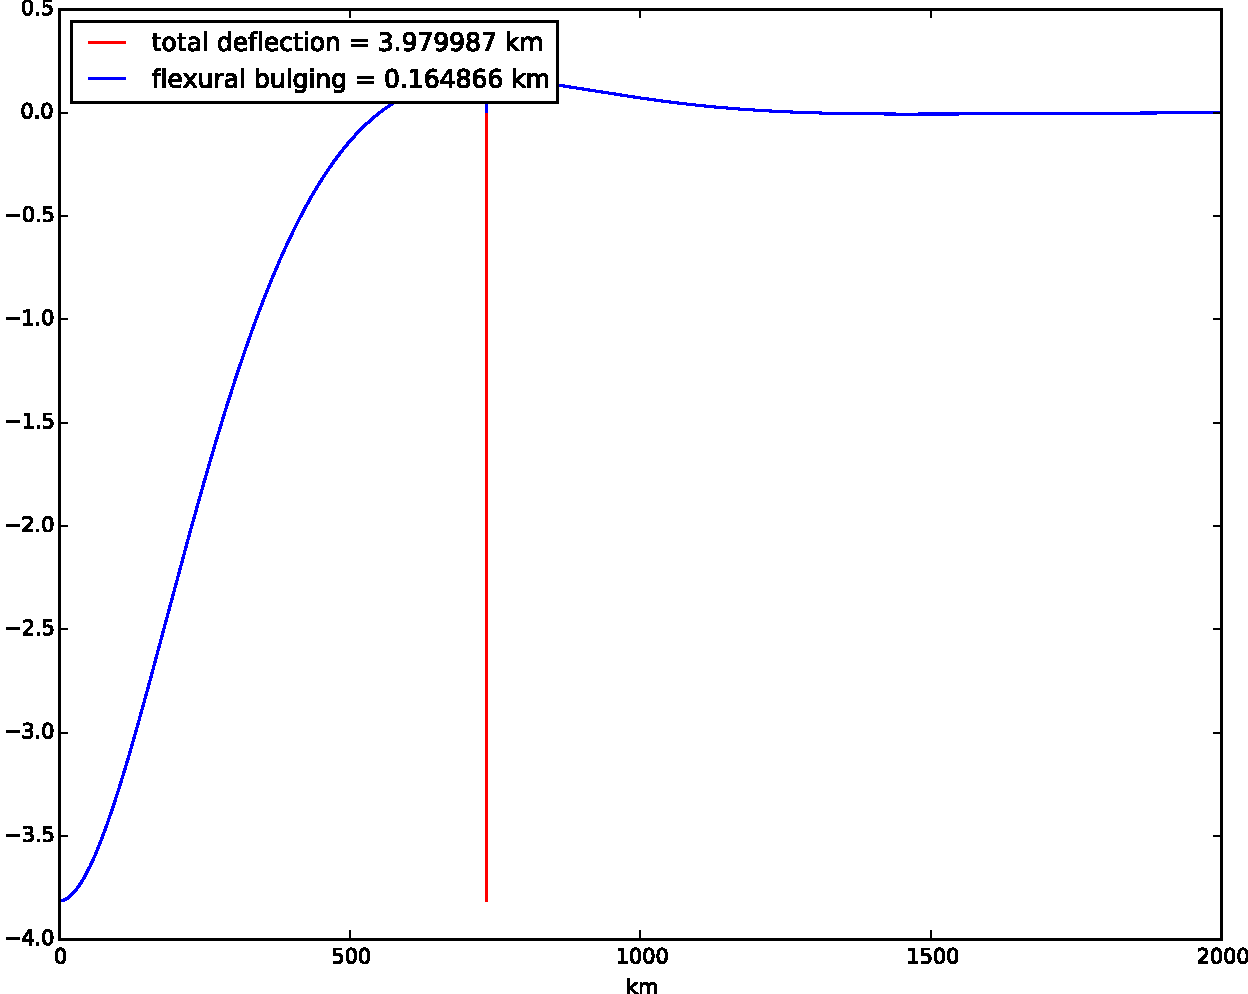
\includegraphics[width=0.65\textwidth]{figures/flex_fig.pdf}
\caption{\footnotesize{Flexural subsidence of the MCR assuming a line load equivalent to sedimentary and volcanic rock $\sim$20 km thick. Other parameters are available in the Appendix.}}
\label{fig:flex_sub}
\end{wrapfigure}

However, the MCR's present narrow structure might not be representative of its pre-Grenville extent, and future models should test the effects of longer wavelength and laterally variable loads.\par

My model also exhibits a flexural bulge nearly 0.5 km in height located $\sim$750 km from the center of the rift (Fig. \ref{fig:flex_sub}). Future analysis should test for potential correlation between this region of positive elevation -- which would be more susceptible to erosion -- with widespread unconformities in the MCR stratigraphy that are currently explained by a ``latent" stage of quiescent rift volcanism.




\section{THERMAL SUBSIDENCE}
\subsection{Previous Studies and Implications}
 
The thermal subsidence of the MCR is highly dependent on mantle temperature since it is essentially a feature of conductive cooling of sublithospheric mantle beneath thinned crust. As significant cooling and subisidence in the region would likely have required the shutoff of tensional stresses or the relocation of the underlying mantle plume, thermal subsidence in the MCR is considered to be largely confined to the later stages of the rift. Using REE inversion techniques to estimate the changing melting depths and temperatures of distinct volcanic sequences in the MCR, \cite{White1997a} estimated the degree of lithospheric thinning at discrete intervals of rifting and suggested the plume source had disappeared by 1094 Ma. In accordance with the thermal subsidence model of \cite{McKenzie1978a}, \cite{White1997a} estimated a $\beta$ stretching factor of 6 in the MCR and elevated mantle temperatures of 1550\textdegree C during the main stage of rift volcanism. This $\beta$ value reconciles the observed subsidence from seismic data with the volcanic volume of the MCR determined by the plume temperature anomaly (Fig. \ref{fig:therm_sub}).\par

\begin{figure}
\noindent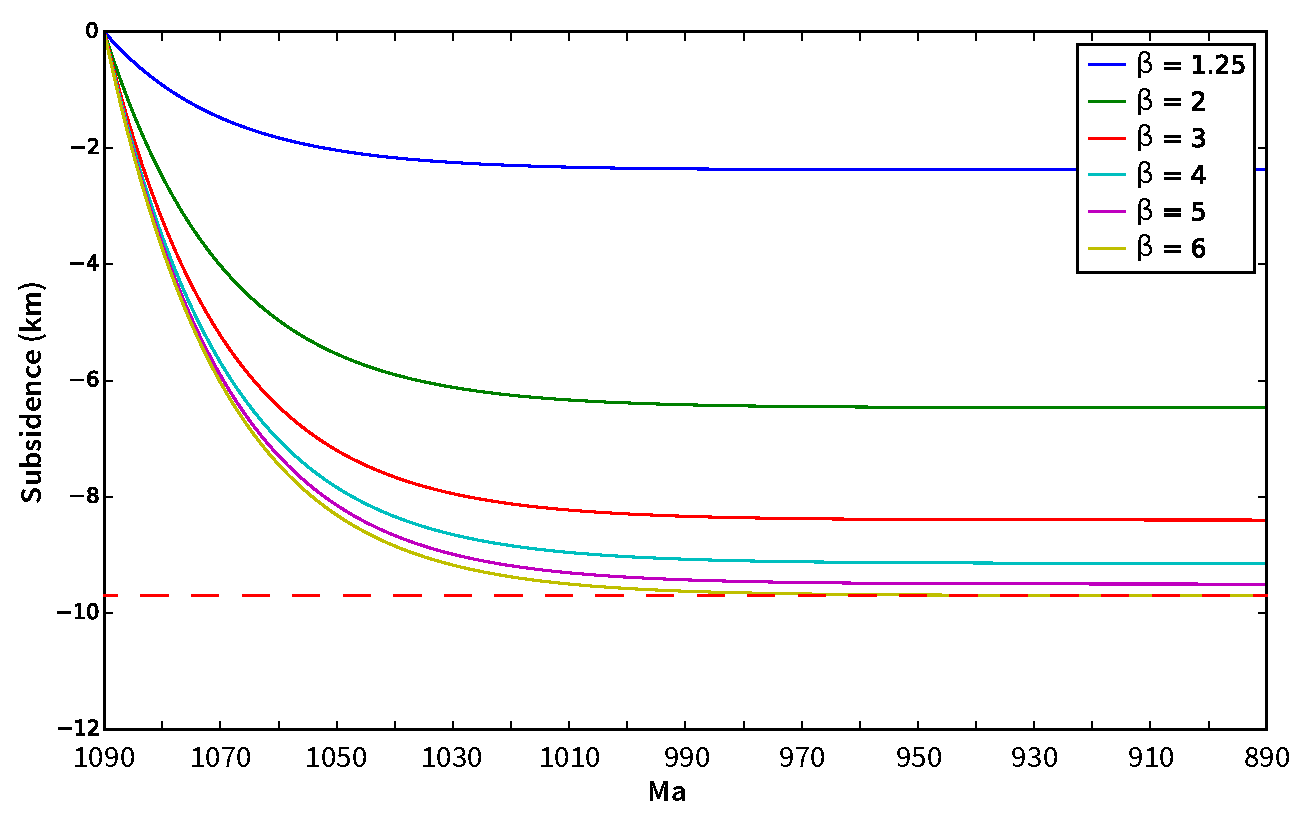
\includegraphics[width=\textwidth]{figures/general_thermal_sub.pdf}
\caption{\footnotesize{Thermal subsidence curves shown for a range of $\beta$ stretching factors. \cite{White1997a} determined that a $\beta$ factor of 6 was most consistent with both the observed subsidence and the volcanic output of the MCR. The diagram above is based on the \cite{McKenzie1978a} stretching model but does not take into account crustal uplift from an upwelling mantle plume as the model of \cite{White1997a} does. The model above therefore illustrates the importance of initial uplift, as it requires at least 2 km to put the final subsidence value in the range estimated from seismic data (4-8 km).}}
\label{fig:therm_sub}
\end{figure}

The duration and degree of thermal subsidence in the MCR is of particular importance because of the lack of current constraints on post-rift sedimentation. \cite{Ojakangas2001a} estimated $\sim$6-10 km of post-rift sedimentation between the Oronto and Bayfield Groups (including highly variable estimates of the Jacobsville Sandstone). The total thickness and provenance of sediment atop MCR volcanics is complicated by the Grenville orogeny, which was underway during or shortly after the end of rift volcanism \citep{Halls2015a}, reversing motion along syn-rift normal faults and interrupting thermal subsidence in the MCR. No comprehensive effort has been made to fully characterize sedimentary sequences in the MCR, and it would be somewhat difficult considering the lack of age constraints on these deposits (as well as the Grenville orogeny) and the largely interpretive aspect of deriving post-rift sediment thickness from seismic data. A comprehensive model of MCR thermal subsidence and the resulting sedimentary basin, when reconciled with future age constraints and seismic data, could largely benefit and clarify this discussion. Do current estimates of sediment thickness exceed what is expected from a thermal subsidence model? Could such discrepancies be explained by the sudden onset of a Grenville compressional regime?

\section{DISCUSSION AND CONCLUSIONS}
\begin{wrapfigure}{l}{0.65\textwidth}
\noindent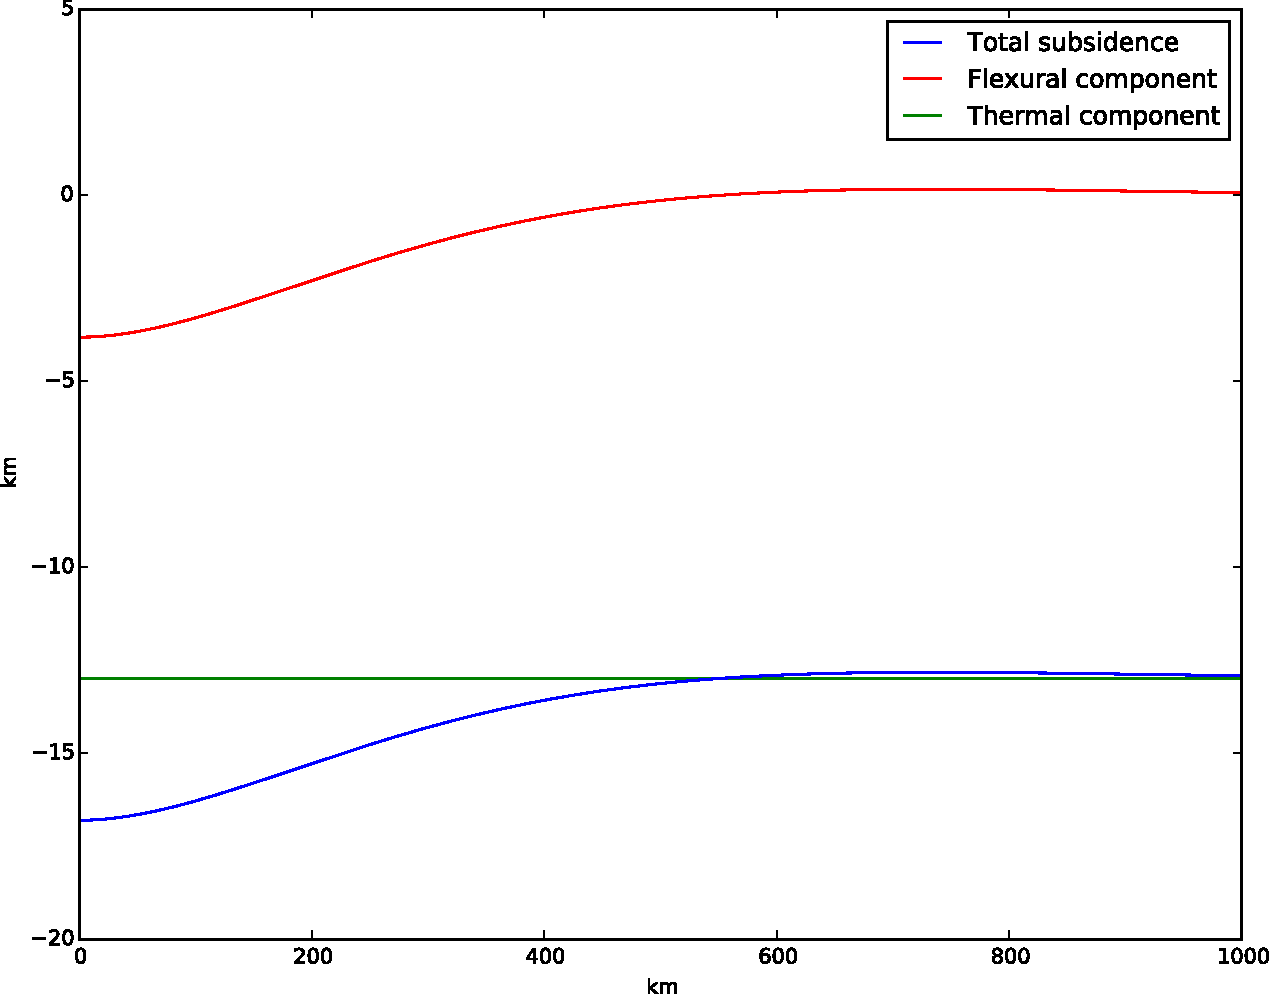
\includegraphics[width=0.65\textwidth]{figures/combined_sub.pdf}
\caption{\footnotesize{Simple summation of flexural and thermal subsidence models. While this is likely an oversimplification of the problem, the result is fairly similar to the $\sim$17 km of lithospheric deflection estimated from seismic data.}}
\label{fig:combined_sub}
\end{wrapfigure}

Summing the total flexural and thermal subsidence in the MCR gives a total deflection of $\sim$17 km. While this simple summation is likely an oversimplification of the combinatory effects of different kinds of subsidence, the final result is in approximate agreement with seismic data, which suggest a total lithospheric deflection of $\sim$20-30 km underneath the MCR \citep{Ojakangas2001a}. Subsidence of this scale, when considering the average thickness of MCR volcanic rock to be $\sim$5.8 km, would necessitate over 10 km of sedimentary infill (up to and above the maximum estimates of \cite{Ojakangas2001a}). Such estimates from models similar to those presented here will be valuable for contextualizing future field measurements.\par

The models above give estimates for long-term subsidence and do not account for changes to the overall stress regime. The subsidence estimates given in this paper could therefore provide a useful reference point for evaluating the timing and severity of the Grenville orogeny. On a broader scale, although this study has not caputured the full complexity of sedimentary basin development, it hopefully provides a unique view of MCR history through the perspective of post-rift development. 
\section*{Appendix}
A Jupyter/IPython notebook with developed code and further text can be viewed at \url{http://nbviewer.ipython.org/github/lfairchild/MCR_subsidence/blob/master/Code/Subsidence_model.ipynb} or directly downloaded from the GitHub repository at \url{https://github.com/lfairchild/MCR_subsidence/tree/master/Code}.



%The Midcontinent Rift (MCR) is a failed rift system that formed within the interior craton of Laurentia (Mesoproterozoic North America) and was active from $\sim$1110 to 1084 Ma. The MCR is notable in both its total volcanic output, which qualifies it as a large igenous province ($\geq$\SI{e5}{km^3} by the criterion of Ernst et al., 2013\nocite{Ernst2013b}), and its geometry, which qualifies it as a rift system. These two characteristics, while present together in the MCR, are not typically associated with each other as they are thought to derive from separate mechanisms. While the volume of volcanic rock in the MCR ($\sim$1-\SI{2e6}{km^3}; \cite{Hutchinson1990a}) necessitates a mantle plume origin, it is unclear whether the plume had any role in the initiation of the rift itself. Recent studies suggest that the MCR formed in response to far-field tectonic stresses as Amazonia rifted from Laurentia, and ended once oceanic spreading between the two continents was successfully established \cite{Stein2014a}. This hypothesis further interprets the MCR as a rift system that coincidentally encountered a mantle plume capable of generating LIP flood basalts, consistent with the idea that the small temperature perturbations ($\sim$100-150\textdegree\ C above normal mantle temperatures) of hotspots can dramatically amplify the decompression magmatism of rift zones \cite{White1989a}. In order to resolve the broad-scale geodynamics of this LIP/rift duality, it becomes important to better understand the wholesale development of the MCR.\par{}
%A widely accepted timeline of MCR development has been inferred through seismic, geochemical, geochronologic and structural measurements \cite{Cannon1989a,Cannon1992b,White1997a,Stein2015a}. However, the post-rift thermal subsidence of the MCR and the development of the resulting sedimentary basin remains a more complicated and contentious storyline. This post-rift stage of final development is critical to inferring past structure from present observations. White (1997)\nocite{White1997a} inferred melting depth from REE inversion techniques, estimating that the lithosphere thinned from an original crustal thickness of 40 km with a $\beta$ stretching factor of 6 \cite{McKenzie1978a}. Significant thermal subsidence in the MCR would likely have been delayed until the hot, buoyant plume source died off, minimizing the subsidence that did occur before its interruption by the $\sim$1080 Ma Grenville Orogeny \cite{White1997a}. The magnitude of the Grenville compressional event may have been underestimated, as new paleomagnetic data suggest a total of 4000 km of crustal shortening \cite{Halls2015a}. Previous models of MCR subsidence should be reevaluated in this context. Flexural models of the MCR, e.g. \cite{Nyquist1988a}, should also be revisited with considerations of longer wavelength loading, potentially greater erosion levels of the surface load, and/or possible correlation between flexural bulges susceptible to erosion and stratigraphic unconformities in the MCR.\par{}
%This study will compile and review the estimates of past investigations of MCR subsidence as well as its broader developmental timeline. This will hopefully allow a comprehensive view of a multifaceted problem, similar to the overview presented by Stein et al. (2015) but with a more quantitative treatment of the MCR's subsidence history. I hope to update certain parameters of past models and reevaluate them in the context of recent work on the MCR. Just as White (1997) showed a buoyant plume and the syn-rift crustal upwarping to likely be responsible for the limited thermal subsidence in the MCR, a thorough review of MCR syn- and post-rift development could prove to have important implications for the larger scale geodynamics of this ancient volcanic structure.

\footnotesize
\bibliographystyle{gsabull}
\bibliography{../../references/allrefs}

\end{document}

